\documentclass[1p]{elsarticle_modified}
%\bibliographystyle{elsarticle-num}

%\usepackage[colorlinks]{hyperref}
%\usepackage{abbrmath_seonhwa} %\Abb, \Ascr, \Acal ,\Abf, \Afrak
\usepackage{amsfonts}
\usepackage{amssymb}
\usepackage{amsmath}
\usepackage{amsthm}
\usepackage{scalefnt}
\usepackage{amsbsy}
\usepackage{kotex}
\usepackage{caption}
\usepackage{subfig}
\usepackage{color}
\usepackage{graphicx}
\usepackage{xcolor} %% white, black, red, green, blue, cyan, magenta, yellow
\usepackage{float}
\usepackage{setspace}
\usepackage{hyperref}

\usepackage{tikz}
\usetikzlibrary{arrows}

\usepackage{multirow}
\usepackage{array} % fixed length table
\usepackage{hhline}

%%%%%%%%%%%%%%%%%%%%%
\makeatletter
\renewcommand*\env@matrix[1][\arraystretch]{%
	\edef\arraystretch{#1}%
	\hskip -\arraycolsep
	\let\@ifnextchar\new@ifnextchar
	\array{*\c@MaxMatrixCols c}}
\makeatother %https://tex.stackexchange.com/questions/14071/how-can-i-increase-the-line-spacing-in-a-matrix
%%%%%%%%%%%%%%%

\usepackage[normalem]{ulem}

\newcommand{\msout}[1]{\ifmmode\text{\sout{\ensuremath{#1}}}\else\sout{#1}\fi}
%SOURCE: \msout is \stkout macro in https://tex.stackexchange.com/questions/20609/strikeout-in-math-mode

\newcommand{\cancel}[1]{
	\ifmmode
	{\color{red}\msout{#1}}
	\else
	{\color{red}\sout{#1}}
	\fi
}

\newcommand{\add}[1]{
	{\color{blue}\uwave{#1}}
}

\newcommand{\replace}[2]{
	\ifmmode
	{\color{red}\msout{#1}}{\color{blue}\uwave{#2}}
	\else
	{\color{red}\sout{#1}}{\color{blue}\uwave{#2}}
	\fi
}

\newcommand{\Sol}{\mathcal{S}} %segment
\newcommand{\D}{D} %diagram
\newcommand{\A}{\mathcal{A}} %arc


%%%%%%%%%%%%%%%%%%%%%%%%%%%%%5 test

\def\sl{\operatorname{\textup{SL}}(2,\Cbb)}
\def\psl{\operatorname{\textup{PSL}}(2,\Cbb)}
\def\quan{\mkern 1mu \triangleright \mkern 1mu}

\theoremstyle{definition}
\newtheorem{thm}{Theorem}[section]
\newtheorem{prop}[thm]{Proposition}
\newtheorem{lem}[thm]{Lemma}
\newtheorem{ques}[thm]{Question}
\newtheorem{cor}[thm]{Corollary}
\newtheorem{defn}[thm]{Definition}
\newtheorem{exam}[thm]{Example}
\newtheorem{rmk}[thm]{Remark}
\newtheorem{alg}[thm]{Algorithm}

\newcommand{\I}{\sqrt{-1}}
\begin{document}

%\begin{frontmatter}
%
%\title{Boundary parabolic representations of knots up to 8 crossings}
%
%%% Group authors per affiliation:
%\author{Yunhi Cho} 
%\address{Department of Mathematics, University of Seoul, Seoul, Korea}
%\ead{yhcho@uos.ac.kr}
%
%
%\author{Seonhwa Kim} %\fnref{s_kim}}
%\address{Center for Geometry and Physics, Institute for Basic Science, Pohang, 37673, Korea}
%\ead{ryeona17@ibs.re.kr}
%
%\author{Hyuk Kim}
%\address{Department of Mathematical Sciences, Seoul National University, Seoul 08826, Korea}
%\ead{hyukkim@snu.ac.kr}
%
%\author{Seokbeom Yoon}
%\address{Department of Mathematical Sciences, Seoul National University, Seoul, 08826,  Korea}
%\ead{sbyoon15@snu.ac.kr}
%
%\begin{abstract}
%We find all boundary parabolic representation of knots up to 8 crossings.
%
%\end{abstract}
%\begin{keyword}
%    \MSC[2010] 57M25 
%\end{keyword}
%
%\end{frontmatter}

%\linenumbers
%\tableofcontents
%
\newcommand\colored[1]{\textcolor{white}{\rule[-0.35ex]{0.8em}{1.4ex}}\kern-0.8em\color{red} #1}%
%\newcommand\colored[1]{\textcolor{white}{ #1}\kern-2.17ex	\textcolor{white}{ #1}\kern-1.81ex	\textcolor{white}{ #1}\kern-2.15ex\color{red}#1	}

{\Large $\underline{12a_{0089}~(K12a_{0089})}$}

\setlength{\tabcolsep}{10pt}
\renewcommand{\arraystretch}{1.6}
\vspace{1cm}\begin{tabular}{m{100pt}>{\centering\arraybackslash}m{274pt}}
\multirow{5}{120pt}{
	\centering
	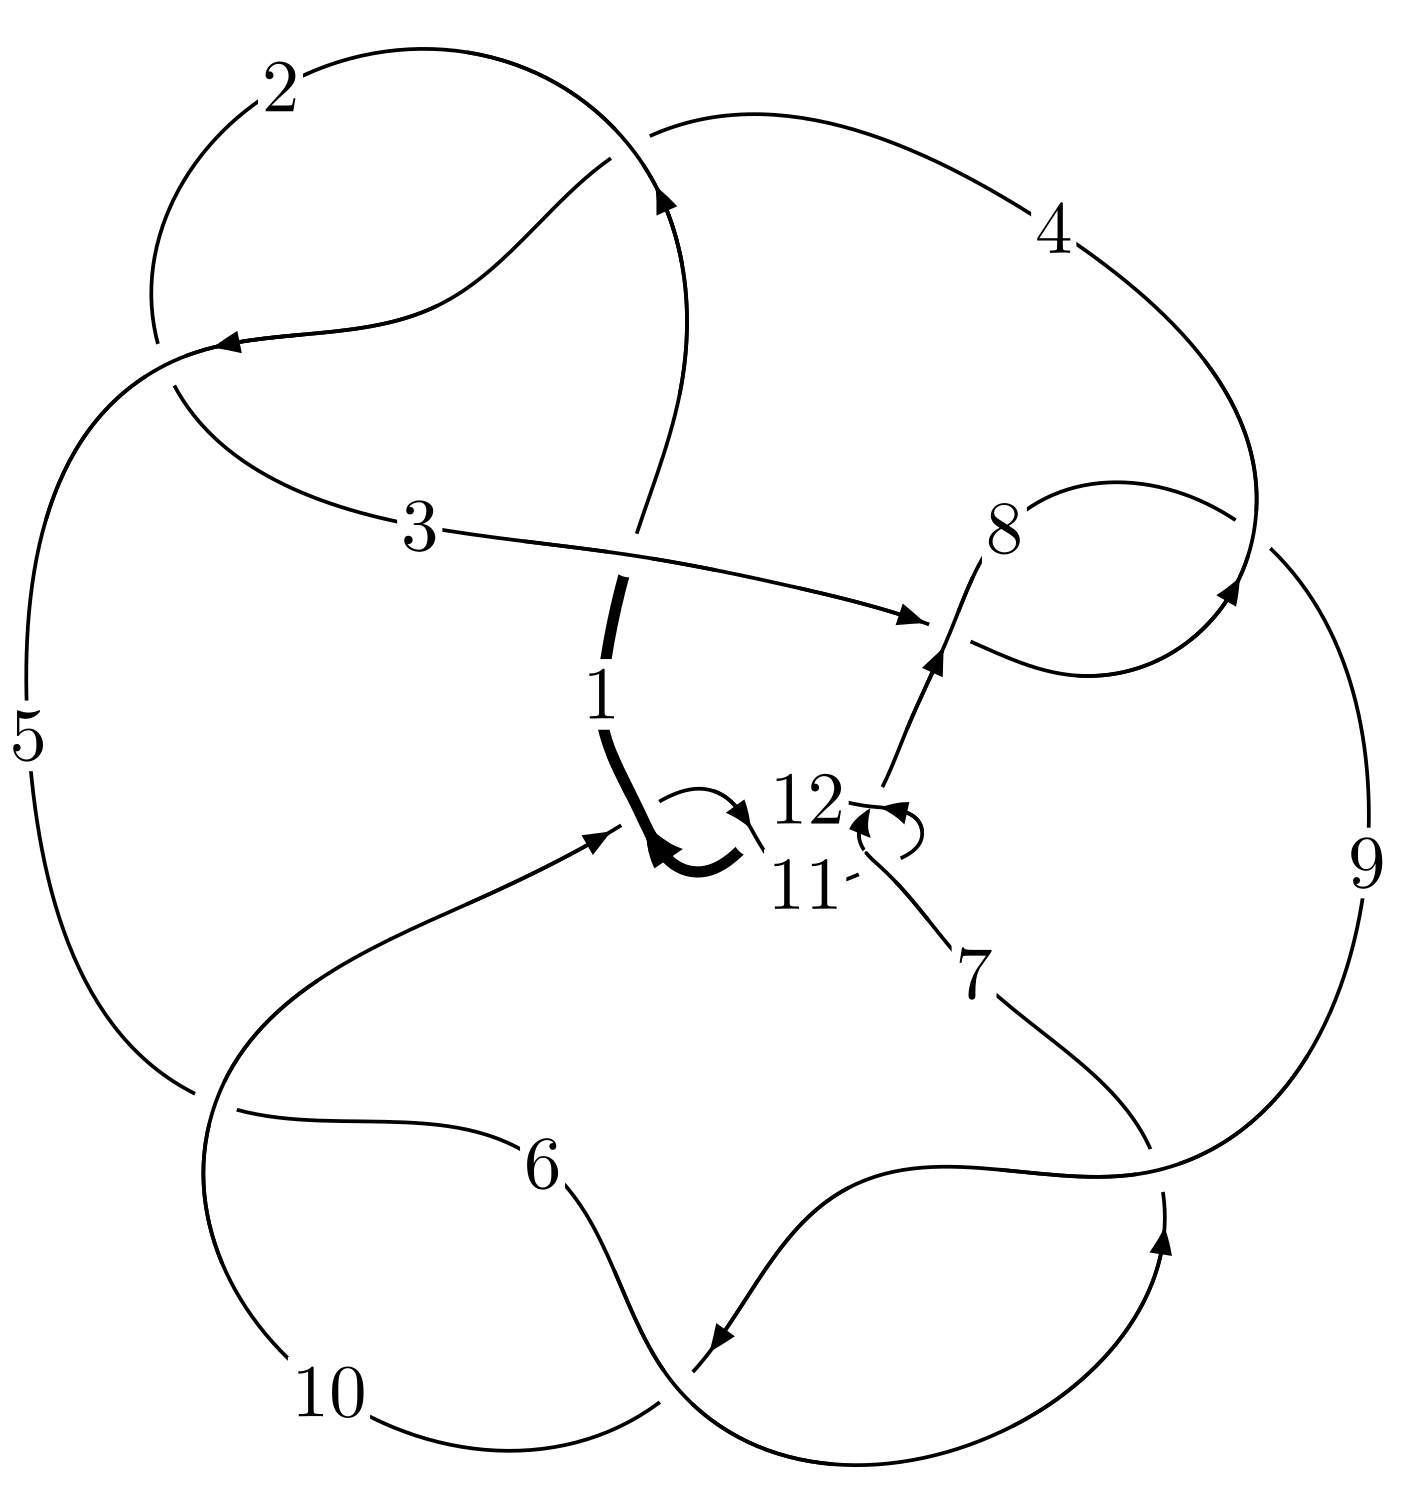
\includegraphics[width=112pt]{../../../GIT/diagram.site/Diagrams/png/890_12a_0089.png}\\
\ \ \ A knot diagram\footnotemark}&
\allowdisplaybreaks
\textbf{Linearized knot diagam} \\
\cline{2-2}
 &
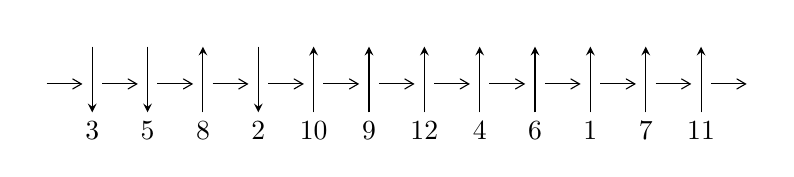
\begin{tikzpicture}[x=20pt, y=17pt]
	% nodes
	\node (C0) at (0, 0) {};
	\node (C1) at (1, 0) {};
	\node (C1U) at (1, +1) {};
	\node (C1D) at (1, -1) {3};

	\node (C2) at (2, 0) {};
	\node (C2U) at (2, +1) {};
	\node (C2D) at (2, -1) {5};

	\node (C3) at (3, 0) {};
	\node (C3U) at (3, +1) {};
	\node (C3D) at (3, -1) {8};

	\node (C4) at (4, 0) {};
	\node (C4U) at (4, +1) {};
	\node (C4D) at (4, -1) {2};

	\node (C5) at (5, 0) {};
	\node (C5U) at (5, +1) {};
	\node (C5D) at (5, -1) {10};

	\node (C6) at (6, 0) {};
	\node (C6U) at (6, +1) {};
	\node (C6D) at (6, -1) {9};

	\node (C7) at (7, 0) {};
	\node (C7U) at (7, +1) {};
	\node (C7D) at (7, -1) {12};

	\node (C8) at (8, 0) {};
	\node (C8U) at (8, +1) {};
	\node (C8D) at (8, -1) {4};

	\node (C9) at (9, 0) {};
	\node (C9U) at (9, +1) {};
	\node (C9D) at (9, -1) {6};

	\node (C10) at (10, 0) {};
	\node (C10U) at (10, +1) {};
	\node (C10D) at (10, -1) {1};

	\node (C11) at (11, 0) {};
	\node (C11U) at (11, +1) {};
	\node (C11D) at (11, -1) {7};

	\node (C12) at (12, 0) {};
	\node (C12U) at (12, +1) {};
	\node (C12D) at (12, -1) {11};
	\node (C13) at (13, 0) {};

	% arrows
	\draw[->,>={angle 60}]
	(C0) edge (C1) (C1) edge (C2) (C2) edge (C3) (C3) edge (C4) (C4) edge (C5) (C5) edge (C6) (C6) edge (C7) (C7) edge (C8) (C8) edge (C9) (C9) edge (C10) (C10) edge (C11) (C11) edge (C12) (C12) edge (C13) ;	\draw[->,>=stealth]
	(C1U) edge (C1D) (C2U) edge (C2D) (C3D) edge (C3U) (C4U) edge (C4D) (C5D) edge (C5U) (C6D) edge (C6U) (C7D) edge (C7U) (C8D) edge (C8U) (C9D) edge (C9U) (C10D) edge (C10U) (C11D) edge (C11U) (C12D) edge (C12U) ;
	\end{tikzpicture} \\
\hhline{~~} \\& 
\textbf{Solving Sequence} \\ \cline{2-2} 
 &
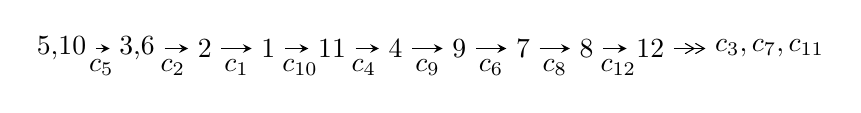
\begin{tikzpicture}[x=23pt, y=7pt]
	% node
	\node (A0) at (-1/8, 0) {5,10};
	\node (A1) at (17/16, 0) {3,6};
	\node (A2) at (17/8, 0) {2};
	\node (A3) at (25/8, 0) {1};
	\node (A4) at (33/8, 0) {11};
	\node (A5) at (41/8, 0) {4};
	\node (A6) at (49/8, 0) {9};
	\node (A7) at (57/8, 0) {7};
	\node (A8) at (65/8, 0) {8};
	\node (A9) at (73/8, 0) {12};
	\node (C1) at (1/2, -1) {$c_{5}$};
	\node (C2) at (13/8, -1) {$c_{2}$};
	\node (C3) at (21/8, -1) {$c_{1}$};
	\node (C4) at (29/8, -1) {$c_{10}$};
	\node (C5) at (37/8, -1) {$c_{4}$};
	\node (C6) at (45/8, -1) {$c_{9}$};
	\node (C7) at (53/8, -1) {$c_{6}$};
	\node (C8) at (61/8, -1) {$c_{8}$};
	\node (C9) at (69/8, -1) {$c_{12}$};
	\node (A10) at (11, 0) {$c_{3},c_{7},c_{11}$};

	% edge
	\draw[->,>=stealth]	
	(A0) edge (A1) (A1) edge (A2) (A2) edge (A3) (A3) edge (A4) (A4) edge (A5) (A5) edge (A6) (A6) edge (A7) (A7) edge (A8) (A8) edge (A9) ;
	\draw[->>,>={angle 60}]	
	(A9) edge (A10);
\end{tikzpicture} \\ 

\end{tabular} \\

\footnotetext{
The image of knot diagram is generated by the software ``\textbf{Draw programme}" developed by Andrew Bartholomew(\url{http://www.layer8.co.uk/maths/draw/index.htm\#Running-draw}), where we modified some parts for our purpose(\url{https://github.com/CATsTAILs/LinksPainter}).
}\phantom \\ \newline 
\centering \textbf{Ideals for irreducible components\footnotemark of $X_{\text{par}}$} 
 
\begin{align*}
I^u_{1}&=\langle 
-2.39749\times10^{215} u^{99}-3.64797\times10^{215} u^{98}+\cdots+1.47790\times10^{217} b-8.18496\times10^{217},\\
\phantom{I^u_{1}}&\phantom{= \langle  }-7.22651\times10^{217} u^{99}-1.52650\times10^{218} u^{98}+\cdots+6.20718\times10^{218} a+5.09074\times10^{219},\\
\phantom{I^u_{1}}&\phantom{= \langle  }u^{100}+2 u^{99}+\cdots-329 u-49\rangle \\
I^u_{2}&=\langle 
1878 a^5 u-2600 a^4 u+\cdots+23830 a-8647,\\
\phantom{I^u_{2}}&\phantom{= \langle  }a^6+3 a^5 u-4 a^5-7 a^4 u- a^4+a^3 u-3 a^3-9 a^2 u+5 a^2+6 a u+2 a- u,\;u^2+1\rangle \\
I^u_{3}&=\langle 
b+1,\;- u^3- u^2+a-3 u-2,\;u^5+u^4+4 u^3+3 u^2+3 u+1\rangle \\
\\
\end{align*}
\raggedright * 3 irreducible components of $\dim_{\mathbb{C}}=0$, with total 117 representations.\\
\footnotetext{All coefficients of polynomials are rational numbers. But the coefficients are sometimes approximated in decimal forms when there is not enough margin.}
\newpage
\renewcommand{\arraystretch}{1}
\centering \section*{I. $I^u_{1}= \langle -2.40\times10^{215} u^{99}-3.65\times10^{215} u^{98}+\cdots+1.48\times10^{217} b-8.18\times10^{217},\;-7.23\times10^{217} u^{99}-1.53\times10^{218} u^{98}+\cdots+6.21\times10^{218} a+5.09\times10^{219},\;u^{100}+2 u^{99}+\cdots-329 u-49 \rangle$}
\flushleft \textbf{(i) Arc colorings}\\
\begin{tabular}{m{7pt} m{180pt} m{7pt} m{180pt} }
\flushright $a_{5}=$&$\begin{pmatrix}1\\0\end{pmatrix}$ \\
\flushright $a_{10}=$&$\begin{pmatrix}0\\u\end{pmatrix}$ \\
\flushright $a_{3}=$&$\begin{pmatrix}0.116422 u^{99}+0.245925 u^{98}+\cdots-89.5951 u-8.20137\\0.0162222 u^{99}+0.0246835 u^{98}+\cdots+12.6540 u+5.53823\end{pmatrix}$ \\
\flushright $a_{6}=$&$\begin{pmatrix}1\\- u^2\end{pmatrix}$ \\
\flushright $a_{2}=$&$\begin{pmatrix}0.132644 u^{99}+0.270609 u^{98}+\cdots-76.9410 u-2.66314\\0.0162222 u^{99}+0.0246835 u^{98}+\cdots+12.6540 u+5.53823\end{pmatrix}$ \\
\flushright $a_{1}=$&$\begin{pmatrix}0.109624 u^{99}+0.205069 u^{98}+\cdots-101.450 u-13.1153\\0.0556512 u^{99}+0.125051 u^{98}+\cdots-32.6639 u-1.40263\end{pmatrix}$ \\
\flushright $a_{11}=$&$\begin{pmatrix}0.0962786 u^{99}+0.162953 u^{98}+\cdots-42.0923 u+2.63606\\-0.0148568 u^{99}-0.0180767 u^{98}+\cdots+15.1895 u+5.87732\end{pmatrix}$ \\
\flushright $a_{4}=$&$\begin{pmatrix}0.0397497 u^{99}+0.138384 u^{98}+\cdots-87.1158 u-19.5365\\0.0202763 u^{99}+0.0752641 u^{98}+\cdots-32.7675 u-4.86979\end{pmatrix}$ \\
\flushright $a_{9}=$&$\begin{pmatrix}- u\\u^3+u\end{pmatrix}$ \\
\flushright $a_{7}=$&$\begin{pmatrix}u^2+1\\- u^4-2 u^2\end{pmatrix}$ \\
\flushright $a_{8}=$&$\begin{pmatrix}0.0290553 u^{99}+0.0399308 u^{98}+\cdots+26.9108 u+15.1478\\-0.0135353 u^{99}-0.0340762 u^{98}+\cdots+44.4150 u+8.98928\end{pmatrix}$ \\
\flushright $a_{12}=$&$\begin{pmatrix}0.109897 u^{99}+0.198612 u^{98}+\cdots-42.6716 u+4.91221\\-0.0101391 u^{99}-0.0246196 u^{98}+\cdots+21.3117 u+6.96002\end{pmatrix}$\\&\end{tabular}
\flushleft \textbf{(ii) Obstruction class $= -1$}\\~\\
\flushleft \textbf{(iii) Cusp Shapes $= 0.216920 u^{99}+0.318284 u^{98}+\cdots-68.3104 u+21.0535$}\\~\\
\newpage\renewcommand{\arraystretch}{1}
\flushleft \textbf{(iv) u-Polynomials at the component}\newline \\
\begin{tabular}{m{50pt}|m{274pt}}
Crossings & \hspace{64pt}u-Polynomials at each crossing \\
\hline $$\begin{aligned}c_{1}\end{aligned}$$&$\begin{aligned}
&u^{100}+50 u^{99}+\cdots+79 u+1
\end{aligned}$\\
\hline $$\begin{aligned}c_{2},c_{4}\end{aligned}$$&$\begin{aligned}
&u^{100}-10 u^{99}+\cdots+11 u-1
\end{aligned}$\\
\hline $$\begin{aligned}c_{3},c_{8}\end{aligned}$$&$\begin{aligned}
&u^{100}+u^{99}+\cdots+224 u+32
\end{aligned}$\\
\hline $$\begin{aligned}c_{5},c_{6},c_{9}\end{aligned}$$&$\begin{aligned}
&u^{100}+2 u^{99}+\cdots-329 u-49
\end{aligned}$\\
\hline $$\begin{aligned}c_{7},c_{11}\end{aligned}$$&$\begin{aligned}
&u^{100}+2 u^{99}+\cdots-15 u-17
\end{aligned}$\\
\hline $$\begin{aligned}c_{10},c_{12}\end{aligned}$$&$\begin{aligned}
&u^{100}-32 u^{99}+\cdots+149 u+289
\end{aligned}$\\
\hline
\end{tabular}\\~\\
\newpage\renewcommand{\arraystretch}{1}
\flushleft \textbf{(v) Riley Polynomials at the component}\newline \\
\begin{tabular}{m{50pt}|m{274pt}}
Crossings & \hspace{64pt}Riley Polynomials at each crossing \\
\hline $$\begin{aligned}c_{1}\end{aligned}$$&$\begin{aligned}
&y^{100}+10 y^{99}+\cdots-2487 y+1
\end{aligned}$\\
\hline $$\begin{aligned}c_{2},c_{4}\end{aligned}$$&$\begin{aligned}
&y^{100}-50 y^{99}+\cdots-79 y+1
\end{aligned}$\\
\hline $$\begin{aligned}c_{3},c_{8}\end{aligned}$$&$\begin{aligned}
&y^{100}-45 y^{99}+\cdots-52736 y+1024
\end{aligned}$\\
\hline $$\begin{aligned}c_{5},c_{6},c_{9}\end{aligned}$$&$\begin{aligned}
&y^{100}+98 y^{99}+\cdots+34251 y+2401
\end{aligned}$\\
\hline $$\begin{aligned}c_{7},c_{11}\end{aligned}$$&$\begin{aligned}
&y^{100}-32 y^{99}+\cdots+149 y+289
\end{aligned}$\\
\hline $$\begin{aligned}c_{10},c_{12}\end{aligned}$$&$\begin{aligned}
&y^{100}+80 y^{99}+\cdots-3531239 y+83521
\end{aligned}$\\
\hline
\end{tabular}\\~\\
\newpage\flushleft \textbf{(vi) Complex Volumes and Cusp Shapes}
$$\begin{array}{c|c|c}  
\text{Solutions to }I^u_{1}& \I (\text{vol} + \sqrt{-1}CS) & \text{Cusp shape}\\
 \hline 
\begin{aligned}
u &= -0.065515 + 0.990541 I \\
a &= -0.41447 + 7.77506 I \\
b &= -1.024690 - 0.010060 I\end{aligned}
 & -3.35320 - 2.04195 I & \phantom{-0.000000 } 0 \\ \hline\begin{aligned}
u &= -0.065515 - 0.990541 I \\
a &= -0.41447 - 7.77506 I \\
b &= -1.024690 + 0.010060 I\end{aligned}
 & -3.35320 + 2.04195 I & \phantom{-0.000000 } 0 \\ \hline\begin{aligned}
u &= -0.969042 + 0.362969 I \\
a &= -0.44792 - 1.56289 I \\
b &= \phantom{-}1.167800 + 0.578024 I\end{aligned}
 & -1.88652 - 12.41730 I & \phantom{-0.000000 } 0 \\ \hline\begin{aligned}
u &= -0.969042 - 0.362969 I \\
a &= -0.44792 + 1.56289 I \\
b &= \phantom{-}1.167800 - 0.578024 I\end{aligned}
 & -1.88652 + 12.41730 I & \phantom{-0.000000 } 0 \\ \hline\begin{aligned}
u &= \phantom{-}0.940871 + 0.436198 I \\
a &= -0.35176 + 1.46851 I \\
b &= \phantom{-}1.145610 - 0.541902 I\end{aligned}
 & -2.76156 + 6.42552 I & \phantom{-0.000000 } 0 \\ \hline\begin{aligned}
u &= \phantom{-}0.940871 - 0.436198 I \\
a &= -0.35176 - 1.46851 I \\
b &= \phantom{-}1.145610 + 0.541902 I\end{aligned}
 & -2.76156 - 6.42552 I & \phantom{-0.000000 } 0 \\ \hline\begin{aligned}
u &= -0.449054 + 0.956643 I \\
a &= \phantom{-}0.757248 - 1.013000 I \\
b &= \phantom{-}0.254382 + 0.493343 I\end{aligned}
 & -1.24139 + 2.42018 I & \phantom{-0.000000 } 0 \\ \hline\begin{aligned}
u &= -0.449054 - 0.956643 I \\
a &= \phantom{-}0.757248 + 1.013000 I \\
b &= \phantom{-}0.254382 - 0.493343 I\end{aligned}
 & -1.24139 - 2.42018 I & \phantom{-0.000000 } 0 \\ \hline\begin{aligned}
u &= -0.246189 + 1.031340 I \\
a &= -0.113223 + 0.585328 I \\
b &= \phantom{-}0.978093 - 0.719756 I\end{aligned}
 & \phantom{-}2.20888 + 3.42556 I & \phantom{-0.000000 } 0 \\ \hline\begin{aligned}
u &= -0.246189 - 1.031340 I \\
a &= -0.113223 - 0.585328 I \\
b &= \phantom{-}0.978093 + 0.719756 I\end{aligned}
 & \phantom{-}2.20888 - 3.42556 I & \phantom{-0.000000 } 0\\
 \hline 
 \end{array}$$\newpage$$\begin{array}{c|c|c}  
\text{Solutions to }I^u_{1}& \I (\text{vol} + \sqrt{-1}CS) & \text{Cusp shape}\\
 \hline 
\begin{aligned}
u &= -0.843566 + 0.298352 I \\
a &= -0.38582 + 1.43354 I \\
b &= \phantom{-}0.289367 - 0.846254 I\end{aligned}
 & \phantom{-}0.73862 - 7.15845 I & \phantom{-0.000000 } 0 \\ \hline\begin{aligned}
u &= -0.843566 - 0.298352 I \\
a &= -0.38582 - 1.43354 I \\
b &= \phantom{-}0.289367 + 0.846254 I\end{aligned}
 & \phantom{-}0.73862 + 7.15845 I & \phantom{-0.000000 } 0 \\ \hline\begin{aligned}
u &= -0.299712 + 1.087720 I \\
a &= \phantom{-}0.278229 - 1.043020 I \\
b &= \phantom{-}0.683576 + 0.775155 I\end{aligned}
 & \phantom{-}3.05539 - 2.19835 I & \phantom{-0.000000 } 0 \\ \hline\begin{aligned}
u &= -0.299712 - 1.087720 I \\
a &= \phantom{-}0.278229 + 1.043020 I \\
b &= \phantom{-}0.683576 - 0.775155 I\end{aligned}
 & \phantom{-}3.05539 + 2.19835 I & \phantom{-0.000000 } 0 \\ \hline\begin{aligned}
u &= \phantom{-}0.764156 + 0.417633 I \\
a &= \phantom{-}0.82151 - 2.08873 I \\
b &= -1.072760 + 0.478965 I\end{aligned}
 & -3.62812 + 6.33519 I & \phantom{-0.000000 } 0 \\ \hline\begin{aligned}
u &= \phantom{-}0.764156 - 0.417633 I \\
a &= \phantom{-}0.82151 + 2.08873 I \\
b &= -1.072760 - 0.478965 I\end{aligned}
 & -3.62812 - 6.33519 I & \phantom{-0.000000 } 0 \\ \hline\begin{aligned}
u &= \phantom{-}0.588441 + 0.632133 I \\
a &= \phantom{-}0.860063 + 0.744032 I \\
b &= -1.160920 - 0.298625 I\end{aligned}
 & -4.41103 - 1.68246 I & \phantom{-0.000000 } 0 \\ \hline\begin{aligned}
u &= \phantom{-}0.588441 - 0.632133 I \\
a &= \phantom{-}0.860063 - 0.744032 I \\
b &= -1.160920 + 0.298625 I\end{aligned}
 & -4.41103 + 1.68246 I & \phantom{-0.000000 } 0 \\ \hline\begin{aligned}
u &= \phantom{-}0.187210 + 1.126150 I \\
a &= \phantom{-}1.048240 + 0.603763 I \\
b &= -0.668387 - 0.373530 I\end{aligned}
 & -1.86846 + 1.01624 I & \phantom{-0.000000 } 0 \\ \hline\begin{aligned}
u &= \phantom{-}0.187210 - 1.126150 I \\
a &= \phantom{-}1.048240 - 0.603763 I \\
b &= -0.668387 + 0.373530 I\end{aligned}
 & -1.86846 - 1.01624 I & \phantom{-0.000000 } 0\\
 \hline 
 \end{array}$$\newpage$$\begin{array}{c|c|c}  
\text{Solutions to }I^u_{1}& \I (\text{vol} + \sqrt{-1}CS) & \text{Cusp shape}\\
 \hline 
\begin{aligned}
u &= -0.680822 + 0.503951 I \\
a &= \phantom{-}0.71326 + 2.08961 I \\
b &= -1.097340 - 0.410444 I\end{aligned}
 & -4.15515 - 0.77241 I & \phantom{-0.000000 } 0 \\ \hline\begin{aligned}
u &= -0.680822 - 0.503951 I \\
a &= \phantom{-}0.71326 - 2.08961 I \\
b &= -1.097340 + 0.410444 I\end{aligned}
 & -4.15515 + 0.77241 I & \phantom{-0.000000 } 0 \\ \hline\begin{aligned}
u &= \phantom{-}0.775959 + 0.333569 I \\
a &= -0.247079 - 1.299000 I \\
b &= \phantom{-}0.253877 + 0.752651 I\end{aligned}
 & -0.16735 + 1.55705 I & \phantom{-0.000000 } 0 \\ \hline\begin{aligned}
u &= \phantom{-}0.775959 - 0.333569 I \\
a &= -0.247079 + 1.299000 I \\
b &= \phantom{-}0.253877 - 0.752651 I\end{aligned}
 & -0.16735 - 1.55705 I & \phantom{-0.000000 } 0 \\ \hline\begin{aligned}
u &= \phantom{-}0.796339 + 0.840767 I \\
a &= -0.413671 - 0.190155 I \\
b &= \phantom{-}1.063020 + 0.436471 I\end{aligned}
 & -3.95267 - 0.55388 I & \phantom{-0.000000 } 0 \\ \hline\begin{aligned}
u &= \phantom{-}0.796339 - 0.840767 I \\
a &= -0.413671 + 0.190155 I \\
b &= \phantom{-}1.063020 - 0.436471 I\end{aligned}
 & -3.95267 + 0.55388 I & \phantom{-0.000000 } 0 \\ \hline\begin{aligned}
u &= -0.670815 + 0.499865 I \\
a &= \phantom{-}0.827036 - 0.598048 I \\
b &= -1.224950 + 0.246355 I\end{aligned}
 & -4.17026 - 3.77857 I & \phantom{-0.000000 } 0 \\ \hline\begin{aligned}
u &= -0.670815 - 0.499865 I \\
a &= \phantom{-}0.827036 + 0.598048 I \\
b &= -1.224950 - 0.246355 I\end{aligned}
 & -4.17026 + 3.77857 I & \phantom{-0.000000 } 0 \\ \hline\begin{aligned}
u &= \phantom{-}0.471451 + 1.064550 I \\
a &= \phantom{-}0.468004 + 0.750338 I \\
b &= \phantom{-}0.586409 - 0.261443 I\end{aligned}
 & -2.12923 + 2.75082 I & \phantom{-0.000000 } 0 \\ \hline\begin{aligned}
u &= \phantom{-}0.471451 - 1.064550 I \\
a &= \phantom{-}0.468004 - 0.750338 I \\
b &= \phantom{-}0.586409 + 0.261443 I\end{aligned}
 & -2.12923 - 2.75082 I & \phantom{-0.000000 } 0\\
 \hline 
 \end{array}$$\newpage$$\begin{array}{c|c|c}  
\text{Solutions to }I^u_{1}& \I (\text{vol} + \sqrt{-1}CS) & \text{Cusp shape}\\
 \hline 
\begin{aligned}
u &= -0.748764 + 0.934617 I \\
a &= -0.435746 + 0.254991 I \\
b &= \phantom{-}1.101640 - 0.489464 I\end{aligned}
 & -3.58978 + 6.56550 I & \phantom{-0.000000 } 0 \\ \hline\begin{aligned}
u &= -0.748764 - 0.934617 I \\
a &= -0.435746 - 0.254991 I \\
b &= \phantom{-}1.101640 + 0.489464 I\end{aligned}
 & -3.58978 - 6.56550 I & \phantom{-0.000000 } 0 \\ \hline\begin{aligned}
u &= \phantom{-}0.545121 + 0.587251 I \\
a &= \phantom{-}0.377482 + 1.297890 I \\
b &= \phantom{-}0.940217 - 0.555672 I\end{aligned}
 & \phantom{-}0.74183 + 4.19177 I & \phantom{-0.000000 } 0. - 6.66805 I \\ \hline\begin{aligned}
u &= \phantom{-}0.545121 - 0.587251 I \\
a &= \phantom{-}0.377482 - 1.297890 I \\
b &= \phantom{-}0.940217 + 0.555672 I\end{aligned}
 & \phantom{-}0.74183 - 4.19177 I & \phantom{-0.000000 -}0. + 6.66805 I \\ \hline\begin{aligned}
u &= -0.681505 + 0.289527 I \\
a &= \phantom{-}0.03851 - 1.94789 I \\
b &= \phantom{-}1.043400 + 0.637281 I\end{aligned}
 & \phantom{-}4.27099 - 6.89948 I & \phantom{-}11.43396 + 7.69737 I \\ \hline\begin{aligned}
u &= -0.681505 - 0.289527 I \\
a &= \phantom{-}0.03851 + 1.94789 I \\
b &= \phantom{-}1.043400 - 0.637281 I\end{aligned}
 & \phantom{-}4.27099 + 6.89948 I & \phantom{-}11.43396 - 7.69737 I \\ \hline\begin{aligned}
u &= -0.721641 + 0.152687 I \\
a &= -0.844995 + 1.089000 I \\
b &= \phantom{-}0.516426 - 0.779174 I\end{aligned}
 & \phantom{-}5.82753 - 1.57926 I & \phantom{-}14.4879 + 1.7882 I \\ \hline\begin{aligned}
u &= -0.721641 - 0.152687 I \\
a &= -0.844995 - 1.089000 I \\
b &= \phantom{-}0.516426 + 0.779174 I\end{aligned}
 & \phantom{-}5.82753 + 1.57926 I & \phantom{-}14.4879 - 1.7882 I \\ \hline\begin{aligned}
u &= -0.082557 + 1.272520 I \\
a &= -1.88035 - 0.05417 I \\
b &= -1.159760 + 0.213440 I\end{aligned}
 & -3.77500 - 2.20981 I & \phantom{-0.000000 } 0 \\ \hline\begin{aligned}
u &= -0.082557 - 1.272520 I \\
a &= -1.88035 + 0.05417 I \\
b &= -1.159760 - 0.213440 I\end{aligned}
 & -3.77500 + 2.20981 I & \phantom{-0.000000 } 0\\
 \hline 
 \end{array}$$\newpage$$\begin{array}{c|c|c}  
\text{Solutions to }I^u_{1}& \I (\text{vol} + \sqrt{-1}CS) & \text{Cusp shape}\\
 \hline 
\begin{aligned}
u &= -0.210143 + 1.259280 I \\
a &= \phantom{-}0.208298 - 0.400854 I \\
b &= \phantom{-}0.395459 - 0.440267 I\end{aligned}
 & -0.98799 + 1.90733 I & \phantom{-0.000000 } 0 \\ \hline\begin{aligned}
u &= -0.210143 - 1.259280 I \\
a &= \phantom{-}0.208298 + 0.400854 I \\
b &= \phantom{-}0.395459 + 0.440267 I\end{aligned}
 & -0.98799 - 1.90733 I & \phantom{-0.000000 } 0 \\ \hline\begin{aligned}
u &= -0.000512 + 1.327390 I \\
a &= -0.130531 + 0.995414 I \\
b &= \phantom{-}0.925020 - 0.921002 I\end{aligned}
 & -0.781932 + 0.661024 I & \phantom{-0.000000 } 0 \\ \hline\begin{aligned}
u &= -0.000512 - 1.327390 I \\
a &= -0.130531 - 0.995414 I \\
b &= \phantom{-}0.925020 + 0.921002 I\end{aligned}
 & -0.781932 - 0.661024 I & \phantom{-0.000000 } 0 \\ \hline\begin{aligned}
u &= \phantom{-}0.609534 + 0.272478 I \\
a &= -0.584068 - 0.350171 I \\
b &= \phantom{-}0.636787 + 0.561311 I\end{aligned}
 & \phantom{-}1.64920 - 0.29233 I & \phantom{-}8.03329 - 0.15871 I \\ \hline\begin{aligned}
u &= \phantom{-}0.609534 - 0.272478 I \\
a &= -0.584068 + 0.350171 I \\
b &= \phantom{-}0.636787 - 0.561311 I\end{aligned}
 & \phantom{-}1.64920 + 0.29233 I & \phantom{-}8.03329 + 0.15871 I \\ \hline\begin{aligned}
u &= -0.092924 + 1.331590 I \\
a &= -0.065930 - 1.068640 I \\
b &= \phantom{-}0.866501 + 0.946140 I\end{aligned}
 & -0.60519 - 6.07717 I & \phantom{-0.000000 } 0 \\ \hline\begin{aligned}
u &= -0.092924 - 1.331590 I \\
a &= -0.065930 + 1.068640 I \\
b &= \phantom{-}0.866501 - 0.946140 I\end{aligned}
 & -0.60519 + 6.07717 I & \phantom{-0.000000 } 0 \\ \hline\begin{aligned}
u &= \phantom{-}0.171260 + 1.324520 I \\
a &= -1.05185 - 1.79678 I \\
b &= -1.035660 + 0.449155 I\end{aligned}
 & -3.23240 + 4.53436 I & \phantom{-0.000000 } 0 \\ \hline\begin{aligned}
u &= \phantom{-}0.171260 - 1.324520 I \\
a &= -1.05185 + 1.79678 I \\
b &= -1.035660 - 0.449155 I\end{aligned}
 & -3.23240 - 4.53436 I & \phantom{-0.000000 } 0\\
 \hline 
 \end{array}$$\newpage$$\begin{array}{c|c|c}  
\text{Solutions to }I^u_{1}& \I (\text{vol} + \sqrt{-1}CS) & \text{Cusp shape}\\
 \hline 
\begin{aligned}
u &= \phantom{-}0.158952 + 1.352890 I \\
a &= \phantom{-}0.057726 - 0.217470 I \\
b &= \phantom{-}0.119895 + 0.688596 I\end{aligned}
 & -3.26940 + 2.41579 I & \phantom{-0.000000 } 0 \\ \hline\begin{aligned}
u &= \phantom{-}0.158952 - 1.352890 I \\
a &= \phantom{-}0.057726 + 0.217470 I \\
b &= \phantom{-}0.119895 - 0.688596 I\end{aligned}
 & -3.26940 - 2.41579 I & \phantom{-0.000000 } 0 \\ \hline\begin{aligned}
u &= -0.270114 + 1.346370 I \\
a &= -0.440781 + 0.149707 I \\
b &= \phantom{-}0.326391 - 0.819413 I\end{aligned}
 & \phantom{-}1.09915 - 5.14819 I & \phantom{-0.000000 } 0 \\ \hline\begin{aligned}
u &= -0.270114 - 1.346370 I \\
a &= -0.440781 - 0.149707 I \\
b &= \phantom{-}0.326391 + 0.819413 I\end{aligned}
 & \phantom{-}1.09915 + 5.14819 I & \phantom{-0.000000 } 0 \\ \hline\begin{aligned}
u &= \phantom{-}0.359092 + 0.487765 I \\
a &= \phantom{-}1.79802 + 1.38487 I \\
b &= -0.343192 - 0.347888 I\end{aligned}
 & -1.57085 + 2.44408 I & \phantom{-}6.62536 - 3.00383 I \\ \hline\begin{aligned}
u &= \phantom{-}0.359092 - 0.487765 I \\
a &= \phantom{-}1.79802 - 1.38487 I \\
b &= -0.343192 + 0.347888 I\end{aligned}
 & -1.57085 - 2.44408 I & \phantom{-}6.62536 + 3.00383 I \\ \hline\begin{aligned}
u &= -0.039784 + 1.394580 I \\
a &= -1.10221 + 0.98947 I \\
b &= -1.170370 - 0.381652 I\end{aligned}
 & -6.92039 - 1.32032 I & \phantom{-0.000000 } 0 \\ \hline\begin{aligned}
u &= -0.039784 - 1.394580 I \\
a &= -1.10221 - 0.98947 I \\
b &= -1.170370 + 0.381652 I\end{aligned}
 & -6.92039 + 1.32032 I & \phantom{-0.000000 } 0 \\ \hline\begin{aligned}
u &= \phantom{-}0.060535 + 0.600233 I \\
a &= \phantom{-}2.03401 - 0.69858 I \\
b &= -0.267096 + 0.124271 I\end{aligned}
 & -1.59835 + 2.35283 I & \phantom{-}6.98886 - 5.08882 I \\ \hline\begin{aligned}
u &= \phantom{-}0.060535 - 0.600233 I \\
a &= \phantom{-}2.03401 + 0.69858 I \\
b &= -0.267096 - 0.124271 I\end{aligned}
 & -1.59835 - 2.35283 I & \phantom{-}6.98886 + 5.08882 I\\
 \hline 
 \end{array}$$\newpage$$\begin{array}{c|c|c}  
\text{Solutions to }I^u_{1}& \I (\text{vol} + \sqrt{-1}CS) & \text{Cusp shape}\\
 \hline 
\begin{aligned}
u &= \phantom{-}0.583705 + 0.093529 I \\
a &= \phantom{-}1.08030 - 2.39263 I \\
b &= -0.837645 + 0.440777 I\end{aligned}
 & \phantom{-}1.17772 + 1.85934 I & \phantom{-}10.62955 - 4.30757 I \\ \hline\begin{aligned}
u &= \phantom{-}0.583705 - 0.093529 I \\
a &= \phantom{-}1.08030 + 2.39263 I \\
b &= -0.837645 - 0.440777 I\end{aligned}
 & \phantom{-}1.17772 - 1.85934 I & \phantom{-}10.62955 + 4.30757 I \\ \hline\begin{aligned}
u &= -0.10232 + 1.46119 I \\
a &= \phantom{-}1.233410 - 0.510771 I \\
b &= \phantom{-}1.064130 + 0.480659 I\end{aligned}
 & -2.93294 - 2.08208 I & \phantom{-0.000000 } 0 \\ \hline\begin{aligned}
u &= -0.10232 - 1.46119 I \\
a &= \phantom{-}1.233410 + 0.510771 I \\
b &= \phantom{-}1.064130 - 0.480659 I\end{aligned}
 & -2.93294 + 2.08208 I & \phantom{-0.000000 } 0 \\ \hline\begin{aligned}
u &= -0.26298 + 1.44481 I \\
a &= \phantom{-}1.06935 - 1.24629 I \\
b &= \phantom{-}1.148140 + 0.579376 I\end{aligned}
 & -1.35388 - 10.35240 I & \phantom{-0.000000 } 0 \\ \hline\begin{aligned}
u &= -0.26298 - 1.44481 I \\
a &= \phantom{-}1.06935 + 1.24629 I \\
b &= \phantom{-}1.148140 - 0.579376 I\end{aligned}
 & -1.35388 + 10.35240 I & \phantom{-0.000000 } 0 \\ \hline\begin{aligned}
u &= -0.530564\phantom{ +0.000000I} \\
a &= \phantom{-}0.408996\phantom{ +0.000000I} \\
b &= -1.19118\phantom{ +0.000000I}\end{aligned}
 & -0.0949506\phantom{ +0.000000I} & \phantom{-}15.0060\phantom{ +0.000000I} \\ \hline\begin{aligned}
u &= \phantom{-}0.17399 + 1.46493 I \\
a &= \phantom{-}0.589969 + 0.807489 I \\
b &= -0.470039 - 0.824556 I\end{aligned}
 & -7.81095 + 4.69129 I & \phantom{-0.000000 } 0 \\ \hline\begin{aligned}
u &= \phantom{-}0.17399 - 1.46493 I \\
a &= \phantom{-}0.589969 - 0.807489 I \\
b &= -0.470039 + 0.824556 I\end{aligned}
 & -7.81095 - 4.69129 I & \phantom{-0.000000 } 0 \\ \hline\begin{aligned}
u &= -0.11054 + 1.47556 I \\
a &= \phantom{-}0.500820 - 0.770357 I \\
b &= -0.381208 + 0.834378 I\end{aligned}
 & -8.30671 + 1.25779 I & \phantom{-0.000000 } 0\\
 \hline 
 \end{array}$$\newpage$$\begin{array}{c|c|c}  
\text{Solutions to }I^u_{1}& \I (\text{vol} + \sqrt{-1}CS) & \text{Cusp shape}\\
 \hline 
\begin{aligned}
u &= -0.11054 - 1.47556 I \\
a &= \phantom{-}0.500820 + 0.770357 I \\
b &= -0.381208 - 0.834378 I\end{aligned}
 & -8.30671 - 1.25779 I & \phantom{-0.000000 } 0 \\ \hline\begin{aligned}
u &= \phantom{-}0.29268 + 1.46125 I \\
a &= -0.402718 - 0.591662 I \\
b &= \phantom{-}0.224404 + 0.986853 I\end{aligned}
 & -5.97166 + 5.43704 I & \phantom{-0.000000 } 0 \\ \hline\begin{aligned}
u &= \phantom{-}0.29268 - 1.46125 I \\
a &= -0.402718 + 0.591662 I \\
b &= \phantom{-}0.224404 - 0.986853 I\end{aligned}
 & -5.97166 - 5.43704 I & \phantom{-0.000000 } 0 \\ \hline\begin{aligned}
u &= -0.33248 + 1.45296 I \\
a &= -0.522607 + 0.612576 I \\
b &= \phantom{-}0.276570 - 1.013290 I\end{aligned}
 & -4.88626 - 11.41650 I & \phantom{-0.000000 } 0 \\ \hline\begin{aligned}
u &= -0.33248 - 1.45296 I \\
a &= -0.522607 - 0.612576 I \\
b &= \phantom{-}0.276570 + 1.013290 I\end{aligned}
 & -4.88626 + 11.41650 I & \phantom{-0.000000 } 0 \\ \hline\begin{aligned}
u &= -0.23283 + 1.49322 I \\
a &= -0.434106 + 0.048242 I \\
b &= -1.39371 + 0.24719 I\end{aligned}
 & -10.62360 - 7.05864 I & \phantom{-0.000000 } 0 \\ \hline\begin{aligned}
u &= -0.23283 - 1.49322 I \\
a &= -0.434106 - 0.048242 I \\
b &= -1.39371 - 0.24719 I\end{aligned}
 & -10.62360 + 7.05864 I & \phantom{-0.000000 } 0 \\ \hline\begin{aligned}
u &= \phantom{-}0.27946 + 1.48522 I \\
a &= -0.35493 - 1.59998 I \\
b &= -1.116750 + 0.624358 I\end{aligned}
 & -9.78659 + 10.13180 I & \phantom{-0.000000 } 0 \\ \hline\begin{aligned}
u &= \phantom{-}0.27946 - 1.48522 I \\
a &= -0.35493 + 1.59998 I \\
b &= -1.116750 - 0.624358 I\end{aligned}
 & -9.78659 - 10.13180 I & \phantom{-0.000000 } 0 \\ \hline\begin{aligned}
u &= -0.23041 + 1.49769 I \\
a &= -0.41694 + 1.47941 I \\
b &= -1.150690 - 0.589914 I\end{aligned}
 & -10.65950 - 4.06737 I & \phantom{-0.000000 } 0\\
 \hline 
 \end{array}$$\newpage$$\begin{array}{c|c|c}  
\text{Solutions to }I^u_{1}& \I (\text{vol} + \sqrt{-1}CS) & \text{Cusp shape}\\
 \hline 
\begin{aligned}
u &= -0.23041 - 1.49769 I \\
a &= -0.41694 - 1.47941 I \\
b &= -1.150690 + 0.589914 I\end{aligned}
 & -10.65950 + 4.06737 I & \phantom{-0.000000 } 0 \\ \hline\begin{aligned}
u &= \phantom{-}0.17781 + 1.50580 I \\
a &= -0.493571 + 0.136163 I \\
b &= -1.372600 - 0.289952 I\end{aligned}
 & -11.32570 + 0.98821 I & \phantom{-0.000000 } 0 \\ \hline\begin{aligned}
u &= \phantom{-}0.17781 - 1.50580 I \\
a &= -0.493571 - 0.136163 I \\
b &= -1.372600 + 0.289952 I\end{aligned}
 & -11.32570 - 0.98821 I & \phantom{-0.000000 } 0 \\ \hline\begin{aligned}
u &= \phantom{-}0.18673 + 1.51693 I \\
a &= \phantom{-}0.937998 + 0.821389 I \\
b &= \phantom{-}1.147980 - 0.495591 I\end{aligned}
 & -6.13141 + 6.86398 I & \phantom{-0.000000 } 0 \\ \hline\begin{aligned}
u &= \phantom{-}0.18673 - 1.51693 I \\
a &= \phantom{-}0.937998 - 0.821389 I \\
b &= \phantom{-}1.147980 + 0.495591 I\end{aligned}
 & -6.13141 - 6.86398 I & \phantom{-0.000000 } 0 \\ \hline\begin{aligned}
u &= -0.38259 + 1.49851 I \\
a &= \phantom{-}0.59734 - 1.46380 I \\
b &= \phantom{-}1.236450 + 0.623365 I\end{aligned}
 & -7.8475 - 17.3020 I & \phantom{-0.000000 } 0 \\ \hline\begin{aligned}
u &= -0.38259 - 1.49851 I \\
a &= \phantom{-}0.59734 + 1.46380 I \\
b &= \phantom{-}1.236450 - 0.623365 I\end{aligned}
 & -7.8475 + 17.3020 I & \phantom{-0.000000 } 0 \\ \hline\begin{aligned}
u &= -0.437376 + 0.101038 I \\
a &= -1.72342 - 0.02563 I \\
b &= \phantom{-}0.743247 - 0.727481 I\end{aligned}
 & \phantom{-}3.35868 + 4.45930 I & \phantom{-}11.81530 - 5.58434 I \\ \hline\begin{aligned}
u &= -0.437376 - 0.101038 I \\
a &= -1.72342 + 0.02563 I \\
b &= \phantom{-}0.743247 + 0.727481 I\end{aligned}
 & \phantom{-}3.35868 - 4.45930 I & \phantom{-}11.81530 + 5.58434 I \\ \hline\begin{aligned}
u &= \phantom{-}0.35136 + 1.52269 I \\
a &= \phantom{-}0.61315 + 1.32966 I \\
b &= \phantom{-}1.237220 - 0.593339 I\end{aligned}
 & -9.0801 + 11.1134 I & \phantom{-0.000000 } 0\\
 \hline 
 \end{array}$$\newpage$$\begin{array}{c|c|c}  
\text{Solutions to }I^u_{1}& \I (\text{vol} + \sqrt{-1}CS) & \text{Cusp shape}\\
 \hline 
\begin{aligned}
u &= \phantom{-}0.35136 - 1.52269 I \\
a &= \phantom{-}0.61315 - 1.32966 I \\
b &= \phantom{-}1.237220 + 0.593339 I\end{aligned}
 & -9.0801 - 11.1134 I & \phantom{-0.000000 } 0 \\ \hline\begin{aligned}
u &= \phantom{-}0.372232\phantom{ +0.000000I} \\
a &= \phantom{-}0.631357\phantom{ +0.000000I} \\
b &= \phantom{-}0.140150\phantom{ +0.000000I}\end{aligned}
 & \phantom{-}0.703212\phantom{ +0.000000I} & \phantom{-}14.5110\phantom{ +0.000000I} \\ \hline\begin{aligned}
u &= -0.168382 + 0.282817 I \\
a &= -0.07085 + 2.51635 I \\
b &= -0.931838 - 0.189422 I\end{aligned}
 & -1.65732 - 0.64432 I & -2.89537 + 1.61582 I \\ \hline\begin{aligned}
u &= -0.168382 - 0.282817 I \\
a &= -0.07085 - 2.51635 I \\
b &= -0.931838 + 0.189422 I\end{aligned}
 & -1.65732 + 0.64432 I & -2.89537 - 1.61582 I \\ \hline\begin{aligned}
u &= -0.05157 + 1.68989 I \\
a &= \phantom{-}0.526136 + 0.107090 I \\
b &= \phantom{-}1.092650 - 0.236274 I\end{aligned}
 & -13.14570 + 3.76638 I & \phantom{-0.000000 } 0 \\ \hline\begin{aligned}
u &= -0.05157 - 1.68989 I \\
a &= \phantom{-}0.526136 - 0.107090 I \\
b &= \phantom{-}1.092650 + 0.236274 I\end{aligned}
 & -13.14570 - 3.76638 I & \phantom{-0.000000 } 0 \\ \hline\begin{aligned}
u &= \phantom{-}0.13501 + 1.69283 I \\
a &= \phantom{-}0.505949 + 0.016872 I \\
b &= \phantom{-}1.038160 + 0.196931 I\end{aligned}
 & -12.85800 + 2.90129 I & \phantom{-0.000000 } 0 \\ \hline\begin{aligned}
u &= \phantom{-}0.13501 - 1.69283 I \\
a &= \phantom{-}0.505949 - 0.016872 I \\
b &= \phantom{-}1.038160 - 0.196931 I\end{aligned}
 & -12.85800 - 2.90129 I & \phantom{-0.000000 } 0 \\ \hline\begin{aligned}
u &= -0.146371 + 0.249725 I \\
a &= \phantom{-}2.79586 - 1.02647 I \\
b &= \phantom{-}0.902300 + 0.690824 I\end{aligned}
 & \phantom{-}2.91057 - 0.92428 I & \phantom{-}11.94422 + 0.25513 I \\ \hline\begin{aligned}
u &= -0.146371 - 0.249725 I \\
a &= \phantom{-}2.79586 + 1.02647 I \\
b &= \phantom{-}0.902300 - 0.690824 I\end{aligned}
 & \phantom{-}2.91057 + 0.92428 I & \phantom{-}11.94422 - 0.25513 I\\
 \hline 
 \end{array}$$\newpage\newpage\renewcommand{\arraystretch}{1}
\centering \section*{II. $I^u_{2}= \langle 1878 a^5 u-2600 a^4 u+\cdots+23830 a-8647,\;3 a^5 u-7 a^4 u+\cdots+5 a^2+2 a,\;u^2+1 \rangle$}
\flushleft \textbf{(i) Arc colorings}\\
\begin{tabular}{m{7pt} m{180pt} m{7pt} m{180pt} }
\flushright $a_{5}=$&$\begin{pmatrix}1\\0\end{pmatrix}$ \\
\flushright $a_{10}=$&$\begin{pmatrix}0\\u\end{pmatrix}$ \\
\flushright $a_{3}=$&$\begin{pmatrix}a\\-0.313575 a^{5} u+0.434129 a^{4} u+\cdots-3.97896 a+1.44381\end{pmatrix}$ \\
\flushright $a_{6}=$&$\begin{pmatrix}1\\1\end{pmatrix}$ \\
\flushright $a_{2}=$&$\begin{pmatrix}-0.313575 a^{5} u+0.434129 a^{4} u+\cdots-2.97896 a+1.44381\\-0.313575 a^{5} u+0.434129 a^{4} u+\cdots-3.97896 a+1.44381\end{pmatrix}$ \\
\flushright $a_{1}=$&$\begin{pmatrix}-0.230422 a^{5} u+0.782267 a^{4} u+\cdots-1.18901 a+0.965103\\0.165136 a^{5} u-0.977292 a^{4} u+\cdots+0.0687928 a+1.64168\end{pmatrix}$ \\
\flushright $a_{11}=$&$\begin{pmatrix}-0.230422 a^{5} u+0.782267 a^{4} u+\cdots-1.18901 a+0.965103\\0.227918 a^{5} u-0.654199 a^{4} u+\cdots+1.66522 a+0.175822\end{pmatrix}$ \\
\flushright $a_{4}=$&$\begin{pmatrix}0.183336 a^{5} u+0.225413 a^{4} u+\cdots+3.74169 a-0.115712\\0.478711 a^{5} u-1.41142 a^{4} u+\cdots+4.04775 a-0.802137\end{pmatrix}$ \\
\flushright $a_{9}=$&$\begin{pmatrix}- u\\0\end{pmatrix}$ \\
\flushright $a_{7}=$&$\begin{pmatrix}0\\1\end{pmatrix}$ \\
\flushright $a_{8}=$&$\begin{pmatrix}-0.0719653 a^{5} u+0.813157 a^{4} u+\cdots+0.816330 a+0.315913\\-0.231758 a^{5} u+0.583904 a^{4} u+\cdots-0.201703 a-0.493071\end{pmatrix}$ \\
\flushright $a_{12}=$&$\begin{pmatrix}-0.230422 a^{5} u+0.782267 a^{4} u+\cdots-1.18901 a+0.965103\\0.458340 a^{5} u-1.43647 a^{4} u+\cdots+2.85423 a-0.789280\end{pmatrix}$\\&\end{tabular}
\flushleft \textbf{(ii) Obstruction class $= 1$}\\~\\
\flushleft \textbf{(iii) Cusp Shapes $= -\frac{5788}{5989} a^5 u-\frac{14428}{5989} a^5-\frac{9080}{5989} a^4 u+\frac{73372}{5989} a^4+\frac{59108}{5989} a^3 u-\frac{39572}{5989} a^3+\frac{20364}{5989} a^2 u+\frac{72864}{5989} a^2+\frac{29264}{5989} a u-\frac{114876}{5989} a-\frac{34044}{5989} u+\frac{50976}{5989}$}\\~\\
\newpage\renewcommand{\arraystretch}{1}
\flushleft \textbf{(iv) u-Polynomials at the component}\newline \\
\begin{tabular}{m{50pt}|m{274pt}}
Crossings & \hspace{64pt}u-Polynomials at each crossing \\
\hline $$\begin{aligned}c_{1}\end{aligned}$$&$\begin{aligned}
&(u^3- u^2+2 u-1)^4
\end{aligned}$\\
\hline $$\begin{aligned}c_{2}\end{aligned}$$&$\begin{aligned}
&(u^3+u^2-1)^4
\end{aligned}$\\
\hline $$\begin{aligned}c_{3},c_{8}\end{aligned}$$&$\begin{aligned}
&(u^6-3 u^4+2 u^2+1)^2
\end{aligned}$\\
\hline $$\begin{aligned}c_{4}\end{aligned}$$&$\begin{aligned}
&(u^3- u^2+1)^4
\end{aligned}$\\
\hline $$\begin{aligned}c_{5},c_{6},c_{9}\end{aligned}$$&$\begin{aligned}
&(u^2+1)^6
\end{aligned}$\\
\hline $$\begin{aligned}c_{7},c_{11}\end{aligned}$$&$\begin{aligned}
&(u^4- u^2+1)^3
\end{aligned}$\\
\hline $$\begin{aligned}c_{10}\end{aligned}$$&$\begin{aligned}
&(u^2+u+1)^6
\end{aligned}$\\
\hline $$\begin{aligned}c_{12}\end{aligned}$$&$\begin{aligned}
&(u^2- u+1)^6
\end{aligned}$\\
\hline
\end{tabular}\\~\\
\newpage\renewcommand{\arraystretch}{1}
\flushleft \textbf{(v) Riley Polynomials at the component}\newline \\
\begin{tabular}{m{50pt}|m{274pt}}
Crossings & \hspace{64pt}Riley Polynomials at each crossing \\
\hline $$\begin{aligned}c_{1}\end{aligned}$$&$\begin{aligned}
&(y^3+3 y^2+2 y-1)^4
\end{aligned}$\\
\hline $$\begin{aligned}c_{2},c_{4}\end{aligned}$$&$\begin{aligned}
&(y^3- y^2+2 y-1)^4
\end{aligned}$\\
\hline $$\begin{aligned}c_{3},c_{8}\end{aligned}$$&$\begin{aligned}
&(y^3-3 y^2+2 y+1)^4
\end{aligned}$\\
\hline $$\begin{aligned}c_{5},c_{6},c_{9}\end{aligned}$$&$\begin{aligned}
&(y+1)^{12}
\end{aligned}$\\
\hline $$\begin{aligned}c_{7},c_{11}\end{aligned}$$&$\begin{aligned}
&(y^2- y+1)^6
\end{aligned}$\\
\hline $$\begin{aligned}c_{10},c_{12}\end{aligned}$$&$\begin{aligned}
&(y^2+y+1)^6
\end{aligned}$\\
\hline
\end{tabular}\\~\\
\newpage\flushleft \textbf{(vi) Complex Volumes and Cusp Shapes}
$$\begin{array}{c|c|c}  
\text{Solutions to }I^u_{2}& \I (\text{vol} + \sqrt{-1}CS) & \text{Cusp shape}\\
 \hline 
\begin{aligned}
u &= \phantom{-0.000000 -}1.000000 I \\
a &= -0.450984 + 1.062990 I \\
b &= \phantom{-}0.877439 - 0.744862 I\end{aligned}
 & \phantom{-}1.37919 + 0.79824 I & \phantom{-}5.50976 + 0.48465 I \\ \hline\begin{aligned}
u &= \phantom{-0.000000 -}1.000000 I \\
a &= \phantom{-}0.696107 - 0.426734 I \\
b &= \phantom{-}0.877439 + 0.744862 I\end{aligned}
 & \phantom{-}1.37919 - 0.79824 I & \phantom{-}5.50976 - 0.48465 I \\ \hline\begin{aligned}
u &= \phantom{-0.000000 -}1.000000 I \\
a &= -0.258387 - 1.162360 I \\
b &= -0.754878\phantom{ +0.000000I}\end{aligned}
 & -2.75839 - 2.02988 I & -1.01951 + 3.46410 I \\ \hline\begin{aligned}
u &= \phantom{-0.000000 -}1.000000 I \\
a &= \phantom{-}0.111295 - 1.400630 I \\
b &= \phantom{-}0.877439 + 0.744862 I\end{aligned}
 & \phantom{-}1.37919 - 4.85801 I & \phantom{-}5.50976 + 6.44355 I \\ \hline\begin{aligned}
u &= \phantom{-0.000000 -}1.000000 I \\
a &= \phantom{-}0.133827 + 0.089093 I \\
b &= \phantom{-}0.877439 - 0.744862 I\end{aligned}
 & \phantom{-}1.37919 + 4.85801 I & \phantom{-}5.50976 - 6.44355 I \\ \hline\begin{aligned}
u &= \phantom{-0.000000 -}1.000000 I \\
a &= \phantom{-}3.76814 - 1.16236 I \\
b &= -0.754878\phantom{ +0.000000I}\end{aligned}
 & -2.75839 + 2.02988 I & -1.01951 - 3.46410 I \\ \hline\begin{aligned}
u &= \phantom{-0.000000 } -1.000000 I \\
a &= -0.450984 - 1.062990 I \\
b &= \phantom{-}0.877439 + 0.744862 I\end{aligned}
 & \phantom{-}1.37919 - 0.79824 I & \phantom{-}5.50976 - 0.48465 I \\ \hline\begin{aligned}
u &= \phantom{-0.000000 } -1.000000 I \\
a &= \phantom{-}0.696107 + 0.426734 I \\
b &= \phantom{-}0.877439 - 0.744862 I\end{aligned}
 & \phantom{-}1.37919 + 0.79824 I & \phantom{-}5.50976 + 0.48465 I \\ \hline\begin{aligned}
u &= \phantom{-0.000000 } -1.000000 I \\
a &= -0.258387 + 1.162360 I \\
b &= -0.754878\phantom{ +0.000000I}\end{aligned}
 & -2.75839 + 2.02988 I & -1.01951 - 3.46410 I \\ \hline\begin{aligned}
u &= \phantom{-0.000000 } -1.000000 I \\
a &= \phantom{-}0.111295 + 1.400630 I \\
b &= \phantom{-}0.877439 - 0.744862 I\end{aligned}
 & \phantom{-}1.37919 + 4.85801 I & \phantom{-}5.50976 - 6.44355 I\\
 \hline 
 \end{array}$$\newpage$$\begin{array}{c|c|c}  
\text{Solutions to }I^u_{2}& \I (\text{vol} + \sqrt{-1}CS) & \text{Cusp shape}\\
 \hline 
\begin{aligned}
u &= \phantom{-0.000000 } -1.000000 I \\
a &= \phantom{-}0.133827 - 0.089093 I \\
b &= \phantom{-}0.877439 + 0.744862 I\end{aligned}
 & \phantom{-}1.37919 - 4.85801 I & \phantom{-}5.50976 + 6.44355 I \\ \hline\begin{aligned}
u &= \phantom{-0.000000 } -1.000000 I \\
a &= \phantom{-}3.76814 + 1.16236 I \\
b &= -0.754878\phantom{ +0.000000I}\end{aligned}
 & -2.75839 - 2.02988 I & -1.01951 + 3.46410 I\\
 \hline 
 \end{array}$$\newpage\newpage\renewcommand{\arraystretch}{1}
\centering \section*{III. $I^u_{3}= \langle b+1,\;- u^3- u^2+a-3 u-2,\;u^5+u^4+4 u^3+3 u^2+3 u+1 \rangle$}
\flushleft \textbf{(i) Arc colorings}\\
\begin{tabular}{m{7pt} m{180pt} m{7pt} m{180pt} }
\flushright $a_{5}=$&$\begin{pmatrix}1\\0\end{pmatrix}$ \\
\flushright $a_{10}=$&$\begin{pmatrix}0\\u\end{pmatrix}$ \\
\flushright $a_{3}=$&$\begin{pmatrix}u^3+u^2+3 u+2\\-1\end{pmatrix}$ \\
\flushright $a_{6}=$&$\begin{pmatrix}1\\- u^2\end{pmatrix}$ \\
\flushright $a_{2}=$&$\begin{pmatrix}u^3+u^2+3 u+1\\-1\end{pmatrix}$ \\
\flushright $a_{1}=$&$\begin{pmatrix}-1\\0\end{pmatrix}$ \\
\flushright $a_{11}=$&$\begin{pmatrix}u\\u\end{pmatrix}$ \\
\flushright $a_{4}=$&$\begin{pmatrix}u^3+u^2+3 u+2\\-1\end{pmatrix}$ \\
\flushright $a_{9}=$&$\begin{pmatrix}- u\\u^3+u\end{pmatrix}$ \\
\flushright $a_{7}=$&$\begin{pmatrix}u^2+1\\- u^4-2 u^2\end{pmatrix}$ \\
\flushright $a_{8}=$&$\begin{pmatrix}- u\\u^3+u\end{pmatrix}$ \\
\flushright $a_{12}=$&$\begin{pmatrix}- u^2-1\\- u^2\end{pmatrix}$\\&\end{tabular}
\flushleft \textbf{(ii) Obstruction class $= 1$}\\~\\
\flushleft \textbf{(iii) Cusp Shapes $= 4 u^4+5 u^3+12 u^2+16 u+8$}\\~\\
\newpage\renewcommand{\arraystretch}{1}
\flushleft \textbf{(iv) u-Polynomials at the component}\newline \\
\begin{tabular}{m{50pt}|m{274pt}}
Crossings & \hspace{64pt}u-Polynomials at each crossing \\
\hline $$\begin{aligned}c_{1},c_{2}\end{aligned}$$&$\begin{aligned}
&(u-1)^5
\end{aligned}$\\
\hline $$\begin{aligned}c_{3},c_{8}\end{aligned}$$&$\begin{aligned}
&u^5
\end{aligned}$\\
\hline $$\begin{aligned}c_{4}\end{aligned}$$&$\begin{aligned}
&(u+1)^5
\end{aligned}$\\
\hline $$\begin{aligned}c_{5},c_{6},c_{10}\end{aligned}$$&$\begin{aligned}
&u^5+u^4+4 u^3+3 u^2+3 u+1
\end{aligned}$\\
\hline $$\begin{aligned}c_{7}\end{aligned}$$&$\begin{aligned}
&u^5+u^4- u^2+u+1
\end{aligned}$\\
\hline $$\begin{aligned}c_{9},c_{12}\end{aligned}$$&$\begin{aligned}
&u^5- u^4+4 u^3-3 u^2+3 u-1
\end{aligned}$\\
\hline $$\begin{aligned}c_{11}\end{aligned}$$&$\begin{aligned}
&u^5- u^4+u^2+u-1
\end{aligned}$\\
\hline
\end{tabular}\\~\\
\newpage\renewcommand{\arraystretch}{1}
\flushleft \textbf{(v) Riley Polynomials at the component}\newline \\
\begin{tabular}{m{50pt}|m{274pt}}
Crossings & \hspace{64pt}Riley Polynomials at each crossing \\
\hline $$\begin{aligned}c_{1},c_{2},c_{4}\end{aligned}$$&$\begin{aligned}
&(y-1)^5
\end{aligned}$\\
\hline $$\begin{aligned}c_{3},c_{8}\end{aligned}$$&$\begin{aligned}
&y^5
\end{aligned}$\\
\hline $$\begin{aligned}c_{5},c_{6},c_{9}\\c_{10},c_{12}\end{aligned}$$&$\begin{aligned}
&y^5+7 y^4+16 y^3+13 y^2+3 y-1
\end{aligned}$\\
\hline $$\begin{aligned}c_{7},c_{11}\end{aligned}$$&$\begin{aligned}
&y^5- y^4+4 y^3-3 y^2+3 y-1
\end{aligned}$\\
\hline
\end{tabular}\\~\\
\newpage\flushleft \textbf{(vi) Complex Volumes and Cusp Shapes}
$$\begin{array}{c|c|c}  
\text{Solutions to }I^u_{3}& \I (\text{vol} + \sqrt{-1}CS) & \text{Cusp shape}\\
 \hline 
\begin{aligned}
u &= -0.233677 + 0.885557 I \\
a &= \phantom{-}1.10636 + 1.69341 I \\
b &= -1.00000\phantom{ +0.000000I}\end{aligned}
 & -3.46474 - 2.21397 I & -0.36497 + 8.87119 I \\ \hline\begin{aligned}
u &= -0.233677 - 0.885557 I \\
a &= \phantom{-}1.10636 - 1.69341 I \\
b &= -1.00000\phantom{ +0.000000I}\end{aligned}
 & -3.46474 + 2.21397 I & -0.36497 - 8.87119 I \\ \hline\begin{aligned}
u &= -0.416284\phantom{ +0.000000I} \\
a &= \phantom{-}0.852303\phantom{ +0.000000I} \\
b &= -1.00000\phantom{ +0.000000I}\end{aligned}
 & -0.762751\phantom{ +0.000000I} & \phantom{-}3.17840\phantom{ +0.000000I} \\ \hline\begin{aligned}
u &= -0.05818 + 1.69128 I \\
a &= -0.532511 + 0.056433 I \\
b &= -1.00000\phantom{ +0.000000I}\end{aligned}
 & -12.60320 - 3.33174 I & \phantom{-}7.77577 + 5.09400 I \\ \hline\begin{aligned}
u &= -0.05818 - 1.69128 I \\
a &= -0.532511 - 0.056433 I \\
b &= -1.00000\phantom{ +0.000000I}\end{aligned}
 & -12.60320 + 3.33174 I & \phantom{-}7.77577 - 5.09400 I\\
 \hline 
 \end{array}$$\newpage
\newpage\renewcommand{\arraystretch}{1}
\centering \section*{ IV. u-Polynomials}
\begin{tabular}{m{50pt}|m{274pt}}
Crossings & \hspace{64pt}u-Polynomials at each crossing \\
\hline $$\begin{aligned}c_{1}\end{aligned}$$&$\begin{aligned}
&((u-1)^5)(u^3- u^2+2 u-1)^4(u^{100}+50 u^{99}+\cdots+79 u+1)
\end{aligned}$\\
\hline $$\begin{aligned}c_{2}\end{aligned}$$&$\begin{aligned}
&((u-1)^5)(u^3+u^2-1)^4(u^{100}-10 u^{99}+\cdots+11 u-1)
\end{aligned}$\\
\hline $$\begin{aligned}c_{3},c_{8}\end{aligned}$$&$\begin{aligned}
&u^5(u^6-3 u^4+2 u^2+1)^2(u^{100}+u^{99}+\cdots+224 u+32)
\end{aligned}$\\
\hline $$\begin{aligned}c_{4}\end{aligned}$$&$\begin{aligned}
&((u+1)^5)(u^3- u^2+1)^4(u^{100}-10 u^{99}+\cdots+11 u-1)
\end{aligned}$\\
\hline $$\begin{aligned}c_{5},c_{6}\end{aligned}$$&$\begin{aligned}
&((u^2+1)^6)(u^5+u^4+\cdots+3 u+1)(u^{100}+2 u^{99}+\cdots-329 u-49)
\end{aligned}$\\
\hline $$\begin{aligned}c_{7}\end{aligned}$$&$\begin{aligned}
&((u^4- u^2+1)^3)(u^5+u^4- u^2+u+1)(u^{100}+2 u^{99}+\cdots-15 u-17)
\end{aligned}$\\
\hline $$\begin{aligned}c_{9}\end{aligned}$$&$\begin{aligned}
&((u^2+1)^6)(u^5- u^4+\cdots+3 u-1)(u^{100}+2 u^{99}+\cdots-329 u-49)
\end{aligned}$\\
\hline $$\begin{aligned}c_{10}\end{aligned}$$&$\begin{aligned}
&(u^2+u+1)^6(u^5+u^4+4 u^3+3 u^2+3 u+1)\\
&\cdot(u^{100}-32 u^{99}+\cdots+149 u+289)
\end{aligned}$\\
\hline $$\begin{aligned}c_{11}\end{aligned}$$&$\begin{aligned}
&((u^4- u^2+1)^3)(u^5- u^4+u^2+u-1)(u^{100}+2 u^{99}+\cdots-15 u-17)
\end{aligned}$\\
\hline $$\begin{aligned}c_{12}\end{aligned}$$&$\begin{aligned}
&(u^2- u+1)^6(u^5- u^4+4 u^3-3 u^2+3 u-1)\\
&\cdot(u^{100}-32 u^{99}+\cdots+149 u+289)
\end{aligned}$\\
\hline
\end{tabular}\newpage\renewcommand{\arraystretch}{1}
\centering \section*{ V. Riley Polynomials}
\begin{tabular}{m{50pt}|m{274pt}}
Crossings & \hspace{64pt}Riley Polynomials at each crossing \\
\hline $$\begin{aligned}c_{1}\end{aligned}$$&$\begin{aligned}
&((y-1)^5)(y^3+3 y^2+2 y-1)^4(y^{100}+10 y^{99}+\cdots-2487 y+1)
\end{aligned}$\\
\hline $$\begin{aligned}c_{2},c_{4}\end{aligned}$$&$\begin{aligned}
&((y-1)^5)(y^3- y^2+2 y-1)^4(y^{100}-50 y^{99}+\cdots-79 y+1)
\end{aligned}$\\
\hline $$\begin{aligned}c_{3},c_{8}\end{aligned}$$&$\begin{aligned}
&y^5(y^3-3 y^2+2 y+1)^4(y^{100}-45 y^{99}+\cdots-52736 y+1024)
\end{aligned}$\\
\hline $$\begin{aligned}c_{5},c_{6},c_{9}\end{aligned}$$&$\begin{aligned}
&(y+1)^{12}(y^5+7 y^4+16 y^3+13 y^2+3 y-1)\\
&\cdot(y^{100}+98 y^{99}+\cdots+34251 y+2401)
\end{aligned}$\\
\hline $$\begin{aligned}c_{7},c_{11}\end{aligned}$$&$\begin{aligned}
&(y^2- y+1)^6(y^5- y^4+4 y^3-3 y^2+3 y-1)\\
&\cdot(y^{100}-32 y^{99}+\cdots+149 y+289)
\end{aligned}$\\
\hline $$\begin{aligned}c_{10},c_{12}\end{aligned}$$&$\begin{aligned}
&(y^2+y+1)^6(y^5+7 y^4+16 y^3+13 y^2+3 y-1)\\
&\cdot(y^{100}+80 y^{99}+\cdots-3531239 y+83521)
\end{aligned}$\\
\hline
\end{tabular}
\vskip 2pc
\end{document}